%%%%%%%%%%%%%%%%%%%%%%%%%%  phdsymp_sample2e.tex %%%%%%%%%%%%%%%%%%%%%%%%%%%%%%
%% changes for phdsymp.cls marked with !PN
%% except all occ. of phdsymp.sty changed phdsymp.cls
%%%%%%%%%%                                                       %%%%%%%%%%%%%
%%%%%%%%%%    More information: see the header of phdsymp.cls   %%%%%%%%%%%%%
%%%%%%%%%%                                                       %%%%%%%%%%%%%
%%%%%%%%%%%%%%%%%%%%%%%%%%%%%%%%%%%%%%%%%%%%%%%%%%%%%%%%%%%%%%%%%%%%%%%%%%%%%%%

%\documentclass[10pt]{phdsymp} %!PN
\documentclass[twocolumn]{phdsymp} %!PN
%\usepackage[top=3cm,bottom=4cm,outer=2cm,inner=3cm]{geometry}
%\documentclass[12pt,draft]{phdsymp} %!PN
%\documentstyle[twocolumn]{phdsymp}
%\documentstyle[12pt,twoside,draft]{phdsymp}
%\documentstyle[9pt,twocolumn,technote,twoside]{phdsymp}

\usepackage[english]{babel}       % Voor nederlandstalige hyphenatie (woordsplitsing)

\usepackage{graphicx}                   % Om figuren te kunnen verwerken
\usepackage{graphics}			% Om figuren te verwerken.
\graphicspath{{figuren/}}               % De plaats waar latex zijn figuren gaat halen.	

\usepackage{times}
\usepackage{subfigure}

\hyphenation{si-mu-la-ted re-a-lis-tic packets really in-clu-ding}

\def\BibTeX{{\rm B\kern-.05em{\sc i\kern-.025em b}\kern-.08em
    T\kern-.1667em\lower.7ex\hbox{E}\kern-.125emX}}

\newtheorem{theorem}{Theorem}


\begin{document}

\title{Indoor mapping with an autonomous quadcopter} %!PN

\author{Karel Serruys}

\supervisor{Joni Dambre, Francis wyffels and Jonas Degrave}

\maketitle

% korte samenvatting van doel en conclusie
\begin{abstract}
This article reports how a custom low-cost indoor quadcopter is optimized and extended to accommodate \textit{Simultaneous Localization and Mapping} (SLAM). First the starting state of the platform is evaluated. Several optimizations have to be made to enable stable autonomous flight behaviour. Optical flow is used to detect drift, PID controllers are used to control the flight behaviour. When the platform has the desired stability, it is extended with a laser range scanner to perform SLAM. Several SLAM methods are considered. Eventually BreezySLAM is chosen. The performance of this algorithm is also evaluated. Finally a platform is obtained both capable of both flying autonomously and mapping its environment.
\end{abstract}

\begin{keywords}
autonomous quadcopter, indoor, optical flow, SLAM
\end{keywords}

\section{Introduction}
The use of quadcopters is increasing in both private and commercial applications. They benefit from a simple mechanical design and thanks to the advances in electronics of the past few years, it can be made easy to control them. In comparison to ground robots, quadcopters can cope well with rough terrain as they only need to fly over it. Quadcopter can be used for tasks that are too dangerous, expensive or infeasible to be done by man. Examples are inspecting a bridge for micro ruptures \cite{paper:structureInspection2}, package delivery \cite{paper:deliveryQuad}, etc. This article focusses on quadcopters for search and rescue missions. Here, quadcopters are used to map a damaged building and to search for survivors.\\
In this article an existing quadcopter platform is evaluated and optimized. When the platform is capable of stable autonomous flight, it is extended to accommodate \textit{Simultaneous Localization and Mapping} (SLAM). With SLAM a map can be made of the quadcopter's environment.

\section{Platform}
The quadcopter platform of W. De Gucht is the starting point of this work \cite{thesis:wouter}. As autopilot, the ArdupilotMega 1.4 is used. The platform also uses a Raspberry Pi to calculate drift based on optical flow. Once drift is detected, the autopilot can make sure it is compensated. The Raspberry Pi is also employed to pass user commands to the autopilot. This platform however lacks the ability to allow safe autonomous flight. To accommodate SLAM, the platform must be equipped with a laser range scanner. The platform is optimized and subsequently extended to allow mapping of its surroundings.

\begin{figure*}[t]
	\centering
	\subfigure[ Map generated without the use of odometry.]{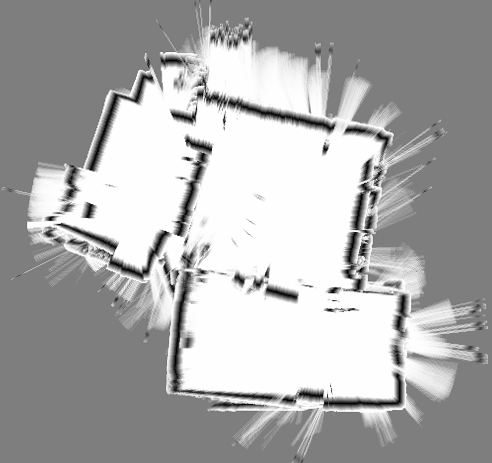
\includegraphics[width=0.4\linewidth]{noodo3ROOMS}}
	\hspace{0.1\linewidth}
	\subfigure[ Map generated using odometry.]{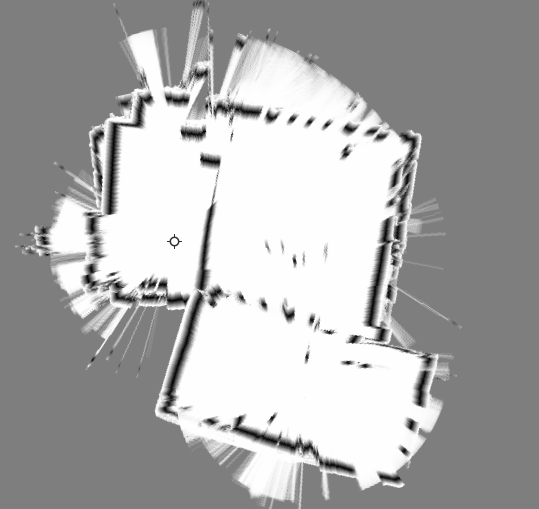
\includegraphics[width=0.4\linewidth]{odo3ROOMS}}
	\caption{This figure show a map of three rooms generated without the use of odometry (a) and with the use of odometry (b). The rooms are more correctly aligned when odometry is used.} \label{fig:SLAM}
\end{figure*}

\subsection{Optimizations}
The Raspberry Pi has a very limited processing power. Optical flow is calculated on the Pi, this leaves very little processing power for anything else. The Raspberry Pi is relieved from the computation of optical flow by using a PC instead. When using the PC the resolution over which optical flow is calculated can be doubled while keeping the same frame rate. This benefits the accuracy of the calculated optical flow. Detecting drift with higher accuracy leads to more accurate drift compensation. As a result the platform will be more stable.\\
Optical flow is calculated by searching features of one frame in a second frame. The accuracy of optical flow is highly dependent on the features selected in the first frame. To further improve the accuracy of drift detection, a different feature detector is proposed. As computational power is no problem on a modern day laptop, the more computationally expensive GFTT detector \cite{paper:GFTT} is implemented. This detector finds optimal features by construction. When comparing optical flow with the GFTT detector to the original FAST detector \cite{paper:FAST}, the use of GFTT clearly performs better, especially when the platform is moving fast and frames become blurry.\\
Next is the height PID controller. The current height is a function of the throttle of the platform. The assumption is made that there exists a throttle which allows the platform to hover. In hover the platform height is constant. Finding this throttle value is not easy as this value is dependent on the battery voltage. The lower the voltage, the higher the throttle value is. The ideal throttle value is estimated during take off by measuring the vertical acceleration of the platform. The error on this estimation needs to be compensated by the integral term of the PID controller. When the estimation error is large, this will take a long time. The correct estimation of the throttle value leads to better height control just after take off. Optimizing the PID parameters according to Ziegler et al. \cite{paper:ZieglerNichols} leads to better height control in later flight.\\
Height control is already a lot better, but there is still quite a bit overshoot. Furthermore fast ascending and descending is bad for stability. This is caused by the fact that optical flow detects drift during ascending and descending that is not actually there. This fake drift leads to an unwanted compensation by the autopilot. To solve this issue, a function generator is proposed. The maximum vertical speed of the platform is limited. When the platform moves slower, the fake drift detected by optical flow is smaller, causing a smaller unwanted compensation and a more stable flight behaviour. The slower vertical movement also reduces the overshoot of the platform.\\
Finally the position controller is looked into. A PI controller is used to control the horizontal speed of the platform. The platform is kept at a certain position by keeping the setpoint of the controller at zero. To move to a specific location in space the velocity in this direction can be augmented until the platform has reached the desired position. The maximum horizontal speed of the platform is also limited to prevent overshoot when the quadcopter moves from one location to another.\\
The platform is now able to fly autonomously and ready to be extended.

\subsection{Extensions}
The platform is extended with a URG-04LX-UG01 laser range scanner. This type of laser range scanner can be connected to one of the USB ports on the Raspberry Pi. However the Raspberry Pi alone is not able to deliver the required current to operate the laser range scanner. To counter this problem the scanner receives extra current from the ArdupilotMega. Now everything is in place to implement a fitting SLAM algorithm.

\section{SLAM}
For SLAM a lot of algorithms exist. The algorithms can be divided into two paradigms \cite{book:SLAMHandbook}. There are those that use extended Kalman filters to estimate the position of the platform and the map points or landmarks. The second paradigm uses particle filters for this estimation. It is essential to know the principles of both paradigms to make a good choice between the two.

\subsection{Extended Kalman filters}
When using extended Kalman filters, the positions of the platform and all the landmarks are assumed to be jointly gaussian distributed. They can be represented by a gaussian variable. This variable is described by its mean vector and a by a covariance matrix. When a new scan is available, the entire mean vector and covariance matrix have to be updated. This is computationally very expensive \cite{paper:FastSLAM}. Moreover, it has been proven that this paradigm can leads to inconsistencies for larger maps \cite{paper:SLAMconsistency}.

\subsection{Particle filters}
The second paradigm uses a number of particles to represent the possible states in which the platform can be. Also, the platform position is assumed to be independent of the landmarks. Consequently landmarks are also independent of each other. The distribution of the landmarks is still assumed to be gaussian. For a 2D map this means that a landmark is described by a mean vector of length two and a 2x2 covariance matrix. The reader can already sense this greatly reduces computational complexity. By grouping the landmarks in a binary tree, the complexity is even further reduced \cite{paper:FastSLAM}.

\begin{figure}[t]
	\centering
	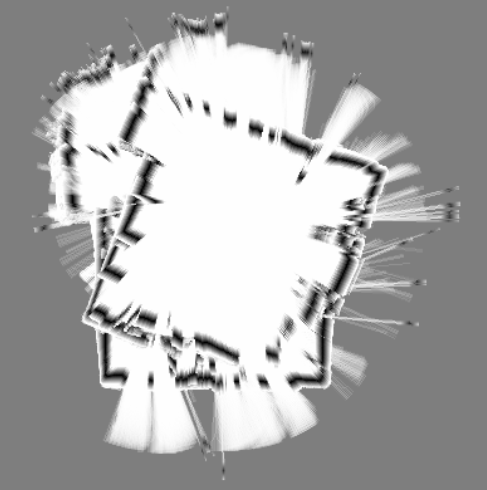
\includegraphics[width=0.8\linewidth]{loopclosure}
	\caption{This figure illustrates the effect of visiting the same location twice. A new map is redrawn above the map that was already there. This is called the loop closing problem.} \label{fig:loopclosing}
\end{figure}

\subsection{BreezySLAM}
From the previous two sections, one can conclude that when looking at computational complexity alone, an algorithm with particle filters needs to be used.\\
First HectorSLAM \cite{paper:hectorSLAM} is looked into. This algorithm uses odometry of all six degrees of freedom a quadcopter has. Implementing it however has failed. Next an attempt has been made to implement TinySLAM \cite{paper:tinySLAM2}, without success, due to its complex interface. Finally BreezySLAM \cite{thesis:BreezySLAM} is implemented, with success. This algorithm is based on TinySLAM. BreezySLAM can also use odometry, but only forward displacement and rotation around the vertical axis are taken into account. This should however not pose any problem as the platform ensures stable flight behaviour.

\section{Integration of SLAM}
Once the SLAM algorithm is chosen, it has to be implemented in the existing architecture of the platform. BreezySLAM can be used both without and with odometry. When mapping multiple rooms, using odometry helps to generate a better map as can be seen in figure \ref{fig:SLAM}. There are still some problems as the algorithm does not perform well when a single location is visited twice. This is illustrated in figure \ref{fig:loopclosing}. In SLAM literature, this is called the loop closing problem \cite{book:SLAMHandbook}.\\
Despite the loop closing problem, the platform is capable of generating a map. This illustrates that the platform is suitable for exploration of unknown environments.

\section{Conclusion}
First of all the quadcopter flight behaviour has been optimized. Drift detection is now more accurate because of the higher resolution of the frames and because of the better GFTT feature detector. By implementing a better height and position control the platform is even more stable. I conclude that the platform is now capable of safe autonomous flight.\\
Second, the platform has been extended with a laser range scanner. By using BreezySLAM the platform is now able to make a relatively accurate map of three rooms. My conclusion is that the platform is capable of mapping a small unknown environment.

\bibliographystyle{IEEEtran}
\bibliography{shortbib}

\end{document}




%%%%%%%%%%%%%%%%%%%%%  End of phdsymp_sample2e.tex  %%%%%%%%%%%%%%%%%%%%%%%%%%%
